\documentclass[twocolumn]{article}

\usepackage{tikz}
\usepackage{amsmath}
\usepackage{csquotes}
\usepackage{booktabs}
\usepackage{biblatex}
\usepackage[plain]{fancyref}

\usepackage{pgfplots}
\pgfplotsset{compat=newest}

\addbibresource{breastCancerDetectionBasedOnNuclearFeatures.bib}

\title{Breast Cancer Detection Based on Nuclear Features}

\author{
  Basant Mahgoub (20180162), Omar Emara (20180364), Hamza Mahmoud(20180214) \\
  Tarik Zaki (20180300), Habiba Yasser (20180188), Mohamed Alkhateb (20180470) \\
  Karim Ashraf (20180424), Mohamed AbdAllah (20180517)
}

\begin{document}

\maketitle

\begin{abstract}

  Breast cancer is one of the fastest growing types of cancer and is one of the
  leading causes of cancer death among women around the globe. Consequently,
  early detection is of essence in death prevention. We present a machine
  learning model for breast cancer detection based on data from Fine Needle
  Aspirations (FNAs). In \Fref{sec:Introduction}, we introduce the concept of
  FNAs and the detection mechanism. In \Fref{sec:Dataset}, we present the
  dataset, discuss the available features, analyse the multicollinearity among
  its features, and investigate the optimal feature selection scheme. In
  \Fref{sec:Implementation}, we present a binary classifier implementation using
  both artificial neural networks and support vector machine models. In
  \Fref{sec:Results}, we present the results of each of the implementations.
  Finally, we conclude in \Fref{sec:Conclusion}.

\end{abstract}

\section{Introduction}
\label{sec:Introduction}

Accurate diagnosis of breast tumor traditionally employed invasive surgical
procedures. However, recent advancements introduced less invasive techniques.
\emph{Fine Needle Aspirations} (FNAs) is a technique whereby a small amount of
tissue is extracted from the tumor without any surgical procedures. The
extracted tissues are investigated under the microscope, looking for the
characteristics of tumor cells that are positively correlated with malignancy.
The physician then makes a decision on the diagnosis, stating the tumor as
benign or malignant.

The process of investigating the tissues is arguably subjective and depends on
the expertise of the physician. Consequently, numerous attempts have done to
automate the classification using regression, linear programming, and machine
learning models. One such attempt is \autocite{Street1993}, where the authors
generated a dataset to aid in fitting classification models based on the
characteristics of tumor cells. The next section explores this dataset.

\section{Dataset}
\label{sec:Dataset}

To generate the dataset described in \autocite{Street1993}, the authors
photographed 569 glass slides stained with a small droplet of fluid extracted
using FNAs. Then, a system was developed to segment each of the cells' nuclei,
accurately capturing its shape and texture. Based on that segmentation, 10
features of the nuclei were computed. Each of which is positively correlated
with malignancy. Finally, for each of the features, the mean, maximum (worst),
and standard error of the feature across all cells in the slide were computed
and stored. The result is a dataset of 569 records and 30 columns. The meaning
of each feature is described in the next section.

\subsection{Nuclear Features}

\begin{itemize}
  \item Radius\\
  The radius of the nucleus, measured by averaging the length of the radial
  lines connecting the center to the segmentation boundary.

  \item Perimeter\\
  The perimeter of the nucleus, measured as the perimeter of the segmentation
  boundary.

  \item Area\\
  The area of the nucleus, measured as the number if pixels inside the
  segmentation plus half for pixels on the segmentation boundary.

  \item Compactness\\
  A measure of the irregularity of the shape of the nucleus, measured using the
  algorithm described in \autocite{Ballard1982} based on the equation
  $P^2 / A$, where $P$ is the perimeter and $A$ is the area. The compactness is
  lowest when the shape is a circular disk and is higher for more irregular
  shapes as demonstrated in \Fref{fig:Compactness}.

  \item Smoothness\\
  A measure of the irregularity of the shape of the nucleus, measured as the
  rate of change of the length of the radial lines connecting the center to the
  segmentation boundary. The smoothness is lowest when the shape is a circular
  disk and is higher for more irregular shapes as demonstrated in
  \Fref{fig:Smoothness}.

  \item Concavity\\
  A measure of the magnitude of cavities or indentation in the shape of the
  nucleus, measured as the length of the small chords that lie outside of
  segmentation boundary. The concavity is lowest when the shape has no cavities
  and is higher for shapes with large cavities as demonstrated in
  \Fref{fig:Concavity}.

  \item Concave Points\\
  A measure of the number of cavities or indentation in the shape of the
  nucleus, measured as the number of cavities in the shape. Similar to
  Concavity but only counts the cavities, regardless of their size.

  \item Symmetry\\
  A measure of the symmetry of the shape of the nucleus, measured as the
  difference in length between both sides of the cords perpendicular to the
  longest chord. The symmetry is lowest for symmetrical shapes and is higher
  for irregular shapes. This is demonstrated in \Fref{fig:Symmetry}.

  \item Fractal Dimension\\
  A measure of the irregularity of the shape of the nucleus, measured as the
  \emph{coastline approximation} described in \autocite{Mandelbrot1982}. The
  fractal dimension is lowest for regular shapes and is higher for irregular
  shapes.

  \item Texture\\
  A measure of the variance of the texture of the nucleus, measured as the
  variance of the gray scale intensities of the nucleus pixels in the
  photograph.
\end{itemize}

\begin{figure}
\begin{center}
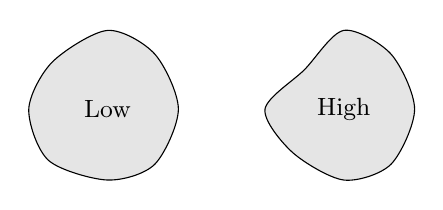
\begin{tikzpicture}[font = \small]
\tikzset{
  blob/.style = {fill = black!10},
}
\draw[blob] plot[smooth cycle] coordinates {(0, 1) (0.6, 0.7) (0.9, 0)
  (0.6, -0.7) (0, -0.9) (-0.75, -0.65) (-1, 0) (-0.7, 0.6)}
  node at (0, 0) {Low};
\draw[blob] plot[smooth cycle, xshift = 3cm] coordinates {(0, 1) (0.6, 0.7)
  (0.9, 0) (0.6, -0.7) (0, -0.9) (-0.65, -0.55) (-1, 0) (-0.5, 0.5)}
  node at (3, 0) {High};
\end{tikzpicture}
\end{center}
\caption{Different compactness values.}
\label{fig:Compactness}
\end{figure}

\begin{figure}
\begin{center}
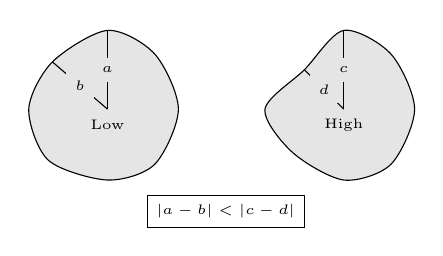
\begin{tikzpicture}[font = \tiny]
\tikzset{
  blob/.style = {fill = black!10},
}
\draw[blob] plot[smooth cycle] coordinates {(0, 1) (0.6, 0.7) (0.9, 0)
  (0.6, -0.7) (0, -0.9) (-0.75, -0.65) (-1, 0) (-0.7, 0.6)}
  node at (0, -0.2) {Low};
\draw (0, 0) -- (0, 1) node [midway, fill=black!10] {$a$};
\draw (0, 0) -- (-0.7, 0.6) node [midway, fill=black!10] {$b$};
\draw[blob] plot[smooth cycle, xshift = 3cm] coordinates {(0, 1) (0.6, 0.7)
  (0.9, 0) (0.6, -0.7) (0, -0.9) (-0.65, -0.55) (-1, 0) (-0.5, 0.5)}
  node at (3, -0.2) {High};
\draw[xshift = 3cm] (0, 0) -- (0, 1) node [midway, fill=black!10] {$c$};
\draw[xshift = 3cm] (0, 0) -- (-0.5, 0.5) node [midway, fill=black!10] {$d$};
\node [draw] at (1.5, -1.3) {$\vert a - b\vert < \vert c - d\vert$};
\end{tikzpicture}
\end{center}
\caption{Different smoothness values.}
\label{fig:Smoothness}
\end{figure}

\begin{figure}
\begin{center}
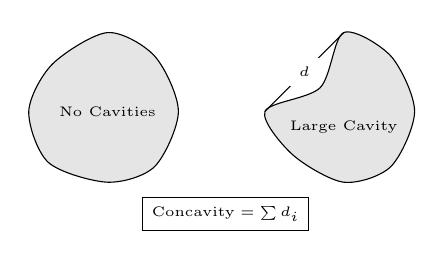
\begin{tikzpicture}[font = \tiny]
\tikzset{
  blob/.style = {fill = black!10},
}
\draw[blob] plot[smooth cycle] coordinates {(0, 1) (0.6, 0.7) (0.9, 0)
  (0.6, -0.7) (0, -0.9) (-0.75, -0.65) (-1, 0) (-0.7, 0.6)}
  node at (0, 0) {No Cavities};
\draw[blob] plot[smooth cycle, xshift = 3cm] coordinates {(0, 1) (0.6, 0.7)
  (0.9, 0) (0.6, -0.7) (0, -0.9) (-0.65, -0.55) (-1, 0) (-0.3, 0.3)}
  node at (3, -0.2) {Large Cavity};
\draw[xshift = 3cm] (0, 1) -- (-1, 0) node [midway, fill=white] {$d$};
\node [draw] at (1.5, -1.3) {$\text{Concavity} = \sum {d_i}$};
\end{tikzpicture}
\end{center}
\caption{Different concavity values.}
\label{fig:Concavity}
\end{figure}

\begin{figure}
\begin{center}
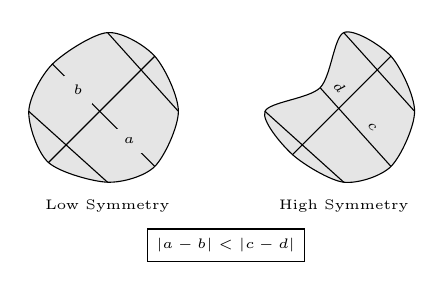
\begin{tikzpicture}[font = \tiny]
\tikzset{
  blob/.style = {fill = black!10},
}
\draw[blob] plot[smooth cycle] coordinates {(0, 1) (0.6, 0.7) (0.9, 0)
  (0.6, -0.7) (0, -0.9) (-0.75, -0.65) (-1, 0) (-0.7, 0.6)}
  node at (0, -1.2) {Low Symmetry};
\draw (0.6, 0.7) -- (-0.75, -0.65);
\draw (-0.7, 0.6) -- (0.6, -0.7)
  node [near end, fill=black!10] {$a$}
  node [near start, fill=black!10] {$b$};
\draw (0, 1) -- (0.9, 0);
\draw (0, -0.9) -- (-1, 0);
\draw[blob] plot[smooth cycle, xshift = 3cm] coordinates {(0, 1) (0.6, 0.7)
  (0.9, 0) (0.6, -0.7) (0, -0.9) (-0.65, -0.55) (-1, 0) (-0.3, 0.3)}
  node at (3, -1.2) {High Symmetry};
\draw[xshift = 3cm] (0.6, 0.7) -- (-0.65, -0.55);
\draw[xshift = 3cm] (-0.3, 0.3) -- (0.6, -0.7)
  node [above, pos = 0.6, sloped] {$c$}
  node [above, pos = 0.12, sloped] {$d$};
\draw[xshift = 3cm] (0, 1) -- (0.9, 0);
\draw[xshift = 3cm] (0, -0.9) -- (-1, 0);
\node [draw] at (1.5, -1.7) {$\vert a - b\vert < \vert c - d\vert$};
\end{tikzpicture}
\end{center}
\caption{Different symmetry values. Note that the symmetry value is lowest when
  the shape is more symmetric and conversely, not the other way around. }
\label{fig:Symmetry}
\end{figure}

\subsection{Features Analysis}

It should be noted that most features measure the irregularities in the shape
of the nucleus, a few features measure the size, and a single feature measure
the color of the nucleus. Indeed, those feature are significant because
according to \autocite{Baba2007}:

\blockquote{ Morphologically, the cancerous cell is characterized by a large
nucleus, having an irregular size and shape, the nucleoli are prominent, the
cytoplasm is scarce and intensely colored or, on the contrary, is pale. }

As mentioned before, for each feature, the mean, maximum (worst), and standard
error across all cells in the slide are computed. The worst values have the most
predictive power against malignancy because only a few cells may exist in a give
sample.

One might note that a lot of the shape features measure the same characteristic
of the nucleus, that is, its shape irregularity. This is intentional to
compensate for the fact that those measures have special cases that may not be
positively correlated with malignancy, so multiple measures are needed. For
instance, elongated nuclei are not signs of malignancy, but they corresponds to
high compactness.

\subsection{Multicollinearity Analysis}

The dataset has no perfect multicollinearity, but the nature of the features
introduces some high multicollinearity that should be considered.

First, some features are largely correlated by definition under certain
assumptions. For instance, assuming sufficiently regular shapes---which is the
case, the radius feature is strongly correlated with both the perimeter and area
features. \Fref{tab:RadiusPerimeterAreaCorrelation} demonstrates this fact by
showing the relevant Pearson correlation coefficients.

\begin{table}
\begin{center}
\begin{tabular}{cccc}
\toprule
 & Radius & Perimeter & Area \\
\midrule
Radius & 1 & 0.997855 & 0.987357 \\
Perimeter & 0.997855 & 1 & 0.986507 \\
Area & 0.987357 & 0.986507 & 1 \\
\bottomrule
\end{tabular}
\end{center}
\caption{Pearson correlation coefficients between the Radius, Perimeter, and
  Area.}
\label{tab:RadiusPerimeterAreaCorrelation}
\end{table}

Second, assuming sufficiently large variance, the mean and maximum of each of
the features are strongly correlated. \Fref{tab:MeanMaxCorrelation}
demonstrates this fact by showing the relevant Pearson correlation coefficients
of some of the features.

\begin{table}
\begin{center}
\begin{tabular}{cc}
\toprule
Mean $\rightarrow$ Max & Pearson correlation coefficients \\
\midrule
Texture & 0.912045 \\
Area & 0.959213 \\
Smoothness & 0.805324 \\
\bottomrule
\end{tabular}
\end{center}
\caption{Pearson correlation coefficients between the mean and max values of
  Texture, Area, and Smoothness.}
\label{tab:MeanMaxCorrelation}
\end{table}

Such significant multicollinearity is undesirable for any fitting problem, but
in practice, it is not an issue because feature selection is typically employed,
which we shall discuss in the next subsection.

\subsection{Feature Selection}

Using a large amount of features when fitting a classifier on a numerical
dataset can lead to overfitting, redundancies, and low predictive accuracy. This
is typically avoided by selecting only a number of relevant features, the
selection being dependent on the problem.

\autocite{Setiono1997} proposed an algorithm to select the most relevant
features using neural networks and evaluated the algorithm on the aforementioned
dataset, the result of which is shown in \Fref{tab:FeatureSelectionAccuracy}.
Even though using all available features produced higher average accuracy across
runs compared to selecting only a number of the features, the predictive
accuracy is actually lower, which means the model is overfitted on the training
data. The authors show similar results on other popular datasets and on
artificially constructed ones.

\begin{table}
\begin{center}
\begin{tabular}{ccc}
\toprule
Average result & Without & With \\
\midrule
Number of features & 9 & 2.7 \\
Accuracy on training set & 100\% & 98.05\% \\
Accuracy on testing set & 93.94\% & 94.15\% \\
\bottomrule
\end{tabular}
\end{center}
\caption{The result of evaluating the feature selection algorithm on the
  dataset. The table shows the training and testing accuracies with and without
  feature selection.}
\label{tab:FeatureSelectionAccuracy}
\end{table}

For this particular dataset, \autocite{Mandelbrot1982} showed that the best
results were obtained using only three features, in particular, the worst area,
the worst smoothness, and the mean texture. This is consistent with the results
shown in \Fref{tab:FeatureSelectionAccuracy}. The author also shows for
prognosis detection that generally, one size feature and one shape feature are
mainly needed, with any other features providing marginal predictive value.

\section{Implementation}
\label{sec:Implementation}

A binary classifier was constructed and trained on the aforementioned dataset
using both an artificial neural network and a support vector machines models.
This section details each of the implementations and evaluation and results of
which are presented in the next section.

\subsection{Artificial Neural Network}

The worst area, worst smoothness, and mean texture features were selected and
loaded from the dataset to be used as the training features. Additionally, the
diagnosis information was loaded from the dataset to be used as the training
reference labels. The features were then normalized to a follow a zero centered
distribution with a unit variance due to the different distributions of each of
the features.

A feed-forward neural network was constructed with two fully connected layers of
128 neurons and a \emph{RELU} activation function. The input layer contains
three neurons corresponding to each of the features and the output layer
contains one neuron corresponding to the binary classification logit value. The
binary cross entropy loss function was used for minimization with a pre analytic
evaluation on a sigmoid function. The \emph{Adam} optimizer was used for
training with a learning rate of $10^{-3}$.

The neural network was fitted with a maximum of 100 epochs and an early stop
condition that monitors the maximum validation binary accuracy with a patience
of 10 epochs. Finally, a 5-fold cross validation was conducted to assess the
generalization of the model, the results of which are presented in
\Fref{sec:Results}.

\subsection{Support Vector Machines}

\section{Results}
\label{sec:Results}

\subsection{Artificial Neural Network}

With 5-fold cross validation, the average binary accuracy was 97.7\%. The
cross validation split corresponding to the median validation binary accuracy
was chosen to evaluate the model on multiple metrics as follows. The binary
confusion matrix is shown in \Fref{tab:NeuralNetworkConfusionMatrix}, the binary
ROC curve is shown in \Fref{fig:NeuralNetworkROC}, and the loss curve across
epochs is shown in \Fref{fig:NeuralNetworkLoss}.

\begin{table}
\begin{center}
\begin{tabular}{ccc}
\toprule
& Positive & Negative \\
\midrule
Positive & 25 & 1 \\
Negative & 1 & 77 \\
\bottomrule
\end{tabular}
\end{center}
\caption{The neural network binary confusion matrix for the cross validation
  split corresponding to the median validation binary accuracy.}
\label{tab:NeuralNetworkConfusionMatrix}
\end{table}

\begin{figure}
\begin{center}
\begin{tikzpicture}
  \begin{axis}[
    title = ROC Curve,
    xlabel = False Positive Rate,
    ylabel = True Positive Rate,
  ]
    \addplot table[x = falsePositiveRate, y = truePositiveRate]
      {neuralNetworkROC.data};
  \end{axis}
\end{tikzpicture}
\end{center}
\caption{The neural network binary ROC curve for the cross validation split
  corresponding to the median validation binary accuracy.}
\label{fig:NeuralNetworkROC}
\end{figure}

\begin{figure}
\begin{center}
\begin{tikzpicture}
  \begin{axis}[
    title = Loss,
    xlabel = Epoch,
    ylabel = Loss,
  ]
    \addplot table[x expr = \coordindex, y = loss] {neuralNetworkLoss.data};
  \end{axis}
\end{tikzpicture}
\end{center}
\caption{The neural network loss curve for the cross validation split
  corresponding to the median validation binary accuracy.}
\label{fig:NeuralNetworkLoss}
\end{figure}

\section{Conclusion}
\label{sec:Conclusion}

\printbibliography

\end{document}
